\section{Introduction}
\label{sec:intro}

% ---- Fig. 1: teaser. TOP ROW: single RGB image -> \method{} ->
% predicted parameters -> editable 3D plant, INCLUDING one edit demo
% (change leaf angle, re-render) — immediately distinguishes this from
% point-cloud completion. BOTTOM STRIP: the difficulty progression,
% isolated -> self-occluded -> neighbor-occluded, with the other input
% modalities (depth / partial PCD) shown as alternative entry points.
% Downstream uses (simulation, trait analytics, compact storage) as
% small icons.
\begin{figure}[t]
  \centering
  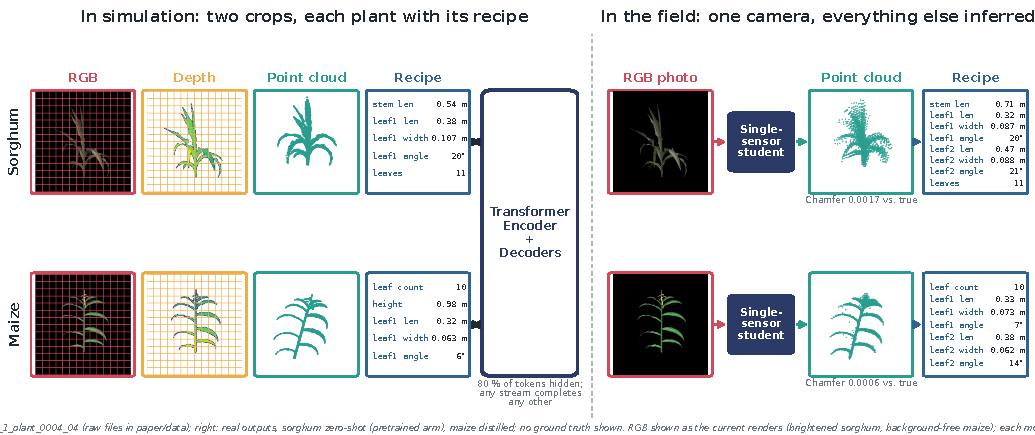
\includegraphics[width=\linewidth]{Figures/fig_teaser.pdf}
  \caption{\textbf{Any sensor in, procedural plant out.} From any subset
  of field-practical modalities (a single photograph, a depth frame, or
  a point cloud truncated by row neighbors), \method{} recovers the full
  procedural representation of the plant: a kilobyte-scale, physiologically
  interpretable parameter set that can be re-rendered to complete geometry,
  used as simulation input, and used for trait analytics at field scale.
  \todo{replace box with figure}}
  \label{fig:teaser}
\end{figure}

% P1 — Goal. (GPS: goal)
Accurate three-dimensional models of individual crop plants enable
high-throughput phenotyping of morphological traits such as leaf angle,
internode length, and canopy architecture, and they are the basis of emerging
agricultural digital twins in which breeding trials run \emph{in
silico}~\citep{hadadi2025procedural, maizefield3d2025}. The representation
best suited to these uses is procedural: a compact set of biologically
interpretable parameters that a generator expands into complete,
editable, simulation-ready geometry~\citep{prusin1990abop,
floraforge2026}. A procedural plant occupies a few kilobytes where a
laser scan occupies megabytes, every parameter corresponds to a trait used by
agronomists, and the model can be edited, re-rendered, and
perturbed in ways that unstructured geometry does not support.
% (fix 2: vision hook — delete the next sentence if unwanted)
Field crops also instantiate a challenge of general interest in 3D
computer vision: recovering a parametric model of a thin, heavily
occluded object from partial multimodal observations.

% P2 — Problem, part 1: existing routes presuppose a rich input. (GPS: problem)
Yet recovering procedural structure from field-acquired sensor data
remains a significant challenge, and every existing route presupposes a
rich, clean observation. Manual parameter specification takes hours per
plant~\citep{floraforge2026}. Staged reconstruction pipelines automate
the process; a recent system annotates laser scans with a
vision-language model and fits a procedural descriptor to
\oldnum{5.4}\,mm median accuracy, but it requires a complete scan of an
isolated plant and roughly ten minutes of computation per
plant~\citep{hadadi2026vlmmaize}. Per-scene optimization methods search
generator parameters against multi-view imagery~\citep{cropcraft2026},
and recent learned models infer parametric plants, but only
from a clean, complete point cloud~\citep{demeter2025,
ghrer2025paramplants}. A phenotyping campaign produces the opposite:
thousands of plants per day, each observed by whichever sensor was
practical (a camera, a depth frame, or a partial scan).

% P3 — Problem, part 2: the geometric frontier. (GPS: problem, sharpened)
In addition, crop plants
are slender: a maize blade is centimeters wide, millimeters thick, and
up to a meter long. In a planted row, each plant is further occluded by
its neighbors, whose leaves interleave with the target; in our field
simulations, roughly a third of the points inside a plant's bounding
region belong to neighboring plants. This regime violates the
assumptions of learned 3D completion: the standard benchmarks contain
compact, largely convex objects and no slender-under-occlusion
category~\citep{yuan2018pcn,yu2021pointr}, and Chamfer distance, the
default metric, is structurally insensitive to thin sheets, so it can
reward reconstructions that miss entire blades~\citep{wu2021dcd,
song2026structural}. Occlusion-aware completion of thin plant organs has begun to address
the input side of this regime, but its output is a completed point
cloud rather than structure~\citep{lee2026occ}.
% TODO-bib: add thinleaf_completion2024 (Plant Phenomics 2024) and
% cornleaf_gridding2023 (Remote Sensing 2023) to CVPR.bib and cite here.
To our knowledge, no prior method recovers a procedural, re-renderable
representation of slender crop organs from a single field-practical
observation (a photograph, a depth frame, or a partial point cloud)
under row-neighbor occlusion: methods that infer plant
parameters require clean, complete scans of isolated
plants~\citep{demeter2025,ghrer2025paramplants}, and methods that
tolerate field occlusion complete unstructured geometry
instead~\citep{lee2026occ}.

% P4 — Solution: the framework. (GPS: solution)
In this work, we present \method{}, a framework that makes this inverse
problem tractable by using the procedural generator itself as the prior.
We pretrain a four-stream masked
autoencoder~\citep{he2022mae,bachmann2022multimae,mizrahi2023fourm,
dong2025embodiedmae} over RGB, depth, point clouds, and tokenized
procedural parameters of \todo{10K--100K} generated maize and sorghum
plants, rendered in simulated rows in which neighboring leaves bend on
contact. Because random modality subsets are masked during pretraining,
a single model learns to complete any subset at inference. A
full-modality teacher is then distilled~\citep{hinton2015distillation}
into single-sensor students for deployment. Distillation
improves cross-modal generation by \oldnum{19.1\%} on average and by
\oldnum{27.5\%} when conditioning on a point cloud alone, and it improves
parameter recovery from that point cloud by \oldnum{43.8\%}.

% P5 — Finding 1: parameters belong at the output.
We also address a design question that arises for any model with access
to generative structure: where should the parameter stream enter? In our
controlled ablations, the parameters are valuable prediction targets but
harm the representation when used as an encoder input. With token budgets
matched, adding the parameter stream to the encoder degrades the frozen
representation on every sorghum phenotype target, and on maize the paired
comparison is a draw. In sorghum, the loss persists in control arms that
restore the sensor-token budget, and it persists even when the parameters
serve only as a reconstruction target for the decoder. Supervising
parameters as a generation target, however, lets the distilled generalist
outperform a parameter-only specialist at parameter regression. One
interpretation, consistent with modality competition~\citep{peng2022ogm}
and negative transfer~\citep{yu2020pcgrad}, is that a stream that already
contains the answer suppresses learning in the streams that must provide the
trait information at test time.

% P6 — Finding 2: metrics.
Chamfer distance ranks depth as the most valuable input
modality (\oldnum{$-32\%$}), whereas a linear probe on the frozen
representation, read out on phenotypic traits, ranks depth within noise
and identifies RGB as the main source of trait information. On slender geometry the two metrics measure
different quantities, surface proximity and recovered structure, and we
adopt the probe as the deciding metric for modality
decisions~\citep{chen2020simclr,wu2021dcd}.

% P7 — Claim + validation + contributions.
We claim that fragmentary field sensing suffices to
recover a complete, interpretable procedural plant, provided the
generator is used for both the training data and the output
representation. We
validate this claim on real field
scans of maize and sorghum with independently reconstructed ground
truth~\citep{maizefield3d2025,hadadi2026vlmmaize}, including rows in
which neighbors occlude the target.
\todo{one sentence of headline real-data results when available.}
The key contributions of this work are:
\begin{enumerate}
  \item \textbf{Task and framework.} The first formulation and system, to
  our knowledge, for recovering procedural plant representations of
  slender, row-occluded field crops from \emph{any subset} of RGB, depth,
  and point-cloud input in one amortized forward pass, with full-modal to
  single-sensor distillation (+\oldnum{19.1\%} generation,
  $-$\oldnum{43.8\%} parameter error from point clouds alone).
  \item \textbf{A design rule for structured modalities.} Controlled,
  budget-matched, two-species evidence that generator parameters are
  valuable prediction targets, while treating them as an auxiliary
  representation-learning modality does not improve, and can degrade,
  the sensor representation; we expect this guidance to transfer to any
  multimodal model with access to privileged generative structure.
  \item \textbf{An evaluation protocol for slender geometry.} A
  demonstration that Chamfer distance and downstream phenotype probes
  disagree systematically on slender organs, and a frozen-latent probe
  protocol that resolves modality decisions where Chamfer is insensitive.
  \item \textbf{A benchmark.} \dataset{}, a two-species procedural
  field benchmark of \todo{N} plants spanning \todo{diversity axes:
  phenotypes / generator configurations / occlusion severities}, with
  paired multimodal captures, physically simulated row occlusion, and
  exact parameter ground truth, together with a real-field evaluation
  split carrying reconstructed procedural ground truth across the
  genotypes of a diversity panel~\citep{maizefield3d2025}. No existing
  dataset combines these elements
  (Tab.~\ref{tab:datacompare})~\citep{schunck2021pheno4d,yuan2018pcn}.
  We will release the data, generation code, and evaluation scripts.
  \todo{confirm release scope and licensing}
\end{enumerate}
